\section{Performance Evaluation}
\subsection{Simulation}
We use a simulation to demonstrate the effectiveness of our cluster-based modal analysis approach along with the clustering strategy. We fix other parameters and only consider the change of the two factors: the network topology and the transmission power \(e_T\). Although in some circumstances, these two factors are correlated, they are independently considered in this simulation. We randomly deploy total of 40 sensor nodes. By adjusting the communication range, we start from a sparse wireless sensor network in which the minimum degree of any nodes in the network is \(p\). Then we consider some conditions when the minimum degree is increased. The energy consumption using four approaches are considered:(1)when all the raw data are streamed back to a sink node (2) when using cluster-based modal analysis with clusters generated from the \(1^{st}\) centralized algorithm (3) from the \(2^{nd}\) centralized algorithm and (4) from the distributed algorithm. Note that in the first approach, the sink node is chosen to be the node whose short path tree (SPT) is the shortest among all the other nodes. Also, no computation energy is included in this approach.

The parameters associated with the simulation are listed in Table \ref{tab:Table2} and the results are shown in Fig. \ref{fig:Simulation2}. It can be seen that for a network with any network degree, using cluster-based approach with optimal clustering, the energy consumption is much smaller compared with that consumed when the raw data are streamed back to a sink node. This conclusion is more evident when the transmission power \(e_T\) is large. For the first approach, the total energy is linearly increased with the increase of \(e_T\) with the slope to be the length of the SPT rooted at the sink node. While in the cluster-based modal analysis, through the optimal clustering, the size of clusters is adjusted to balance the energy consumed in wireless communication and in modal analysis computation. Note that the optimal cluster size is not affected by network topology. In a dense network, it is more possible to achieve the obtained optimal cluster size and therefore, the total energy will be lower than a network with sparse connectivity. The optimal cluster sizes used in these two centralized algorithms are illustrated in Table \ref{tab:simulation}. 
\begin{table}
	\centering
\begin{tabular}{|c|c|c|c|c|c|}
\hline
\(e_T(mAh)\)&\(5e-4\)&\(1e-3\)&\(1.5e-3\)&\(2e-3\)&\(2.5e-3\)\\
\hline
\(n_{opt}\) for Alg. 1&\(6\)&\(7\)&\(8\)&\(9\)&\(10\)\\
\hline
\(n_{opt}\) for Alg. 2&\(3\) &\(5\)&\(6\)&\(7\)&\(8\)\\
\hline
\end{tabular}
	\caption{Parameters used in Fig. \ref{fig:Simulation2}}
	\label{tab:simulation}
\end{table}

\begin{figure}
	\centering
		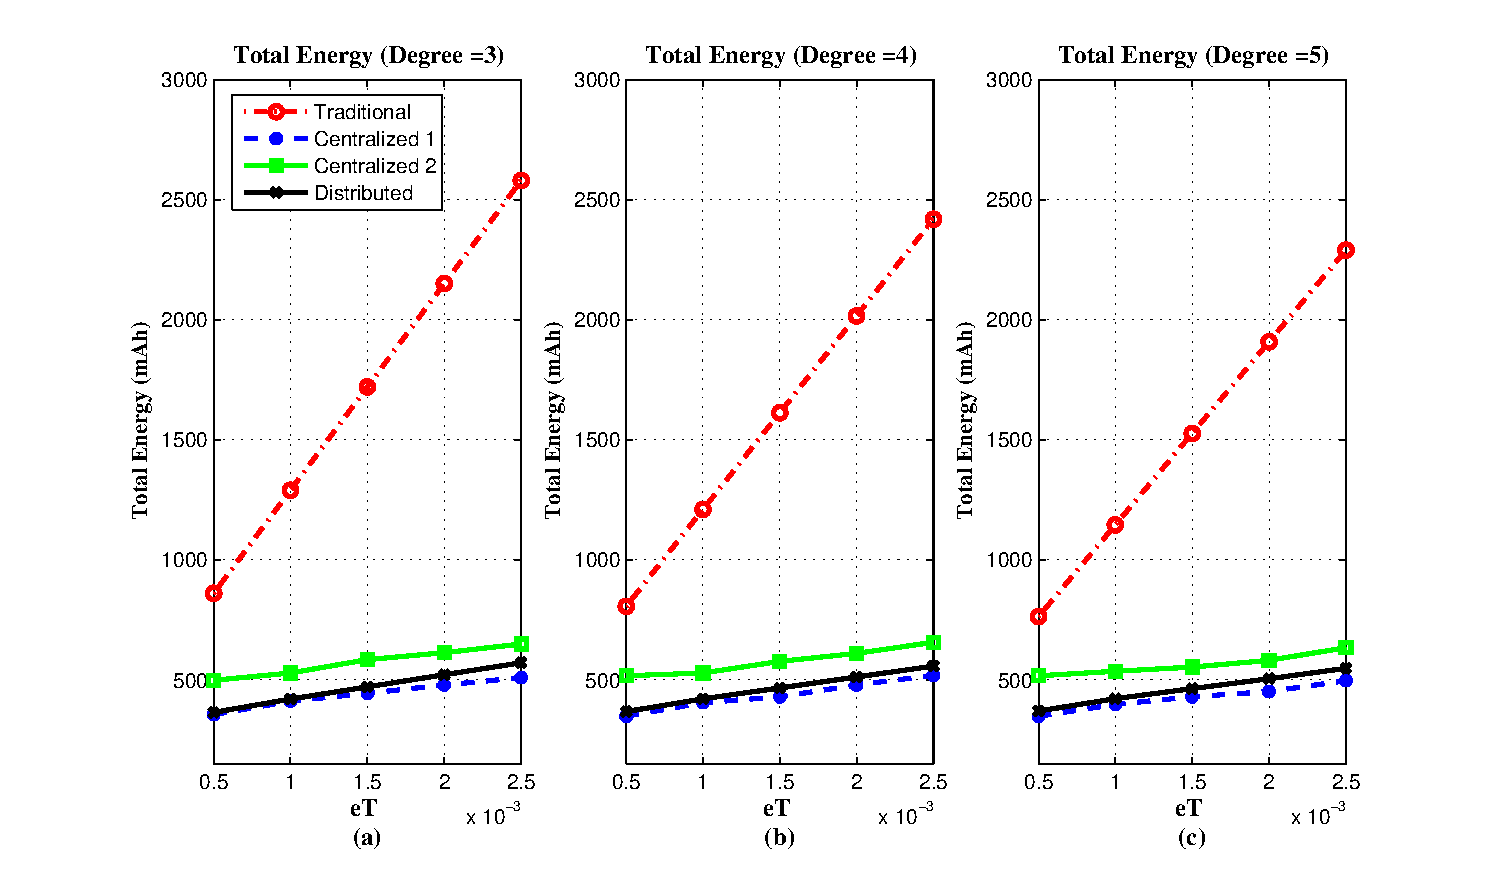
\includegraphics[width=.49\textwidth,height=.25\textwidth]{Simulation2.eps}
	\caption{The Total Energy in Different Scenarios. (a)Network Degree=3 (b)Network Degree=4 (c) Network Degree=5}
	\label{fig:Simulation2}
\end{figure}

To further demonstrate the importance of optimal cluster size, we illustrate the energy consumption of the cluster-based modal analysis in which clusters are obtained from the \(1^{st}\) centralized algorithm but with different cluster sizes beside optimal one (see Fig. 12). It can be seen that compared with other cluster sizes, clustering using designed optimal cluster size can achieve lower overall energy consumption. 

\subsection{Implementation}
We are going to test the effectiveness of our cluster-based modal analysis approach through a real implementation. The wireless sensor nodes adopted are particularly developed by us for general SHM applications (see Fig.\ref{fig:SHMMote}). This type of node is called the SHM Mote and is developed based on Intel Imote2 [ref] which has a much faster on-board processor and much larger RAM space compared to other off-the-shelf smart sensor platforms. Particularly, each SHM Mote also includes a sensor board to accommodate various sensors in SHM applications, a 32Mb non-volatile memory space to store the sampled data, an AM radio transmitter/receiver for synchronized sensing, and a RF amplifiers to increase the communication range (up to 300 meters). 

The SHM Motes run modified TinyOS and are configured to sample the accelerometer in a synchronized manner at frequency of 512Hz. Fig. \ref{fig:Structure}(a) shows the setting of the lab test. The test building has 13 floors, at each floor, a mote is deployed to monitor the structure's horizontal vibration. We adjust the transmission power to be \(e_T =\) in this test after a few tests on link-quality. Under this transmission power, the topology of the network is illustrated in \ref{fig:Structure}(b). We use a gateway node which is connected a computer for the control purpose, while this gateway can be removed in future implementation. Under the command of gateway, each Mote starts collecting \(N = 10752\) data samples synchronously. Sensor nodes are then partitioned into multiple clusters. The cluster information is calculated by the centralized algorithms run in the computer and then is feed to each node through wireless link. Once each node has the cluster information, the cluster-based modal analysis is implemented in each cluster, one cluster at a time, to identify the first three mode shapes of the structure.  The obtained mode shapes of each cluster are then aggregated to the gateway.  For comparison, traditional approach is also used in which all measured data are transmitted the gateway. The ERA using all the measurement data in a batch to identify the mode shapes of the whole structure

Fig. \ref{fig:modeshapes}(a) and (b) illustrates the identified mode shapes by our cluster-based modal analysis. It can be seen that using cluster-based modal analysis, the mode shapes can be identified without losing much of the accuracy compared with the traditional centralized approach. Moreover, the energy communication cost is decreased from \( 1000mAh\) to \(500mAh\).
